\documentclass[12pt]{article}
\usepackage[letterpaper, margin=1in]{geometry}
\usepackage{graphicx}
\usepackage{subcaption}
\graphicspath{{./Figures/}}
\usepackage{hyperref}
\usepackage{parskip}
\usepackage{amsmath}
\usepackage[framed, numbered]{matlab-prettifier}
\lstset{inputpath=../}
\usepackage{titlesec}
\usepackage{gensymb}

\titleformat*{\section}{\large\bfseries}
%\allowdisplaybreaks

% remove vertical spacing above top figure
\makeatletter
\setlength{\@fptop}{0pt}
\makeatother
%

\title{ELECENG 3CL4 Lab 5 Report}
\author{
    Aaron Pinto \\
    pintoa9 \\
    L02
    \and
    Raeed Hassan \\
    hassam41 \\
    L02
}

\begin{document}

\maketitle
\clearpage

\section{Design of a Lead-Lag Compensator for the Quanser Servomotor}
The design of the lead-lag compensator uses the lead compensator that was designed in Lab 4, and modifies it to reach a steady-state error target without affecting the transient response significantly. This is achieved by introducing a lag compensator with the addition of an additional pole and zero. The zero was placed at 0.2, a point close to the origin. As the design objective of the lag compensator is to reduce the steady state error due a step disturbance by a factor of 10, the pole is placed at $z/10 = 0.02$. The angle between the zero and pole relative to the closed-loop pole was found to be 0.52 degrees, below the 1 degree design guideline. This lag compensator is simply added in series to the existing lead compensator. The addition of the lag compensator in MATLAB can be seen in Listing~\ref{listing:lag}.

\lstinputlisting[style=Matlab-editor, caption={Lag compensator}, label={listing:lag}, firstline=69, lastline=81, firstnumber=69]{lab5.m}

The addition of the lag compensator does not have a significant effect on the transient performance of the system, as seen in the root locus in Figure~\ref{fig:rlocus}, the step response in Figure~\ref{fig:step}, and the ramp response in Figure~\ref{fig:ramp}.

The addition of the lag compensator significantly reduces the steady state error of the system, as seen in the response to a step disturbance in Figure~\ref{fig:dist}. The steady state error in the system with the lead-lag compensator is about 10\% of the error in the system with just a lead compensator. The steady state error design objective of the lead-lag compensator is achieved, while also keeping the transient response that is designed with the lead compensator largely unchanged.

\begin{figure}[h]
    \centering
    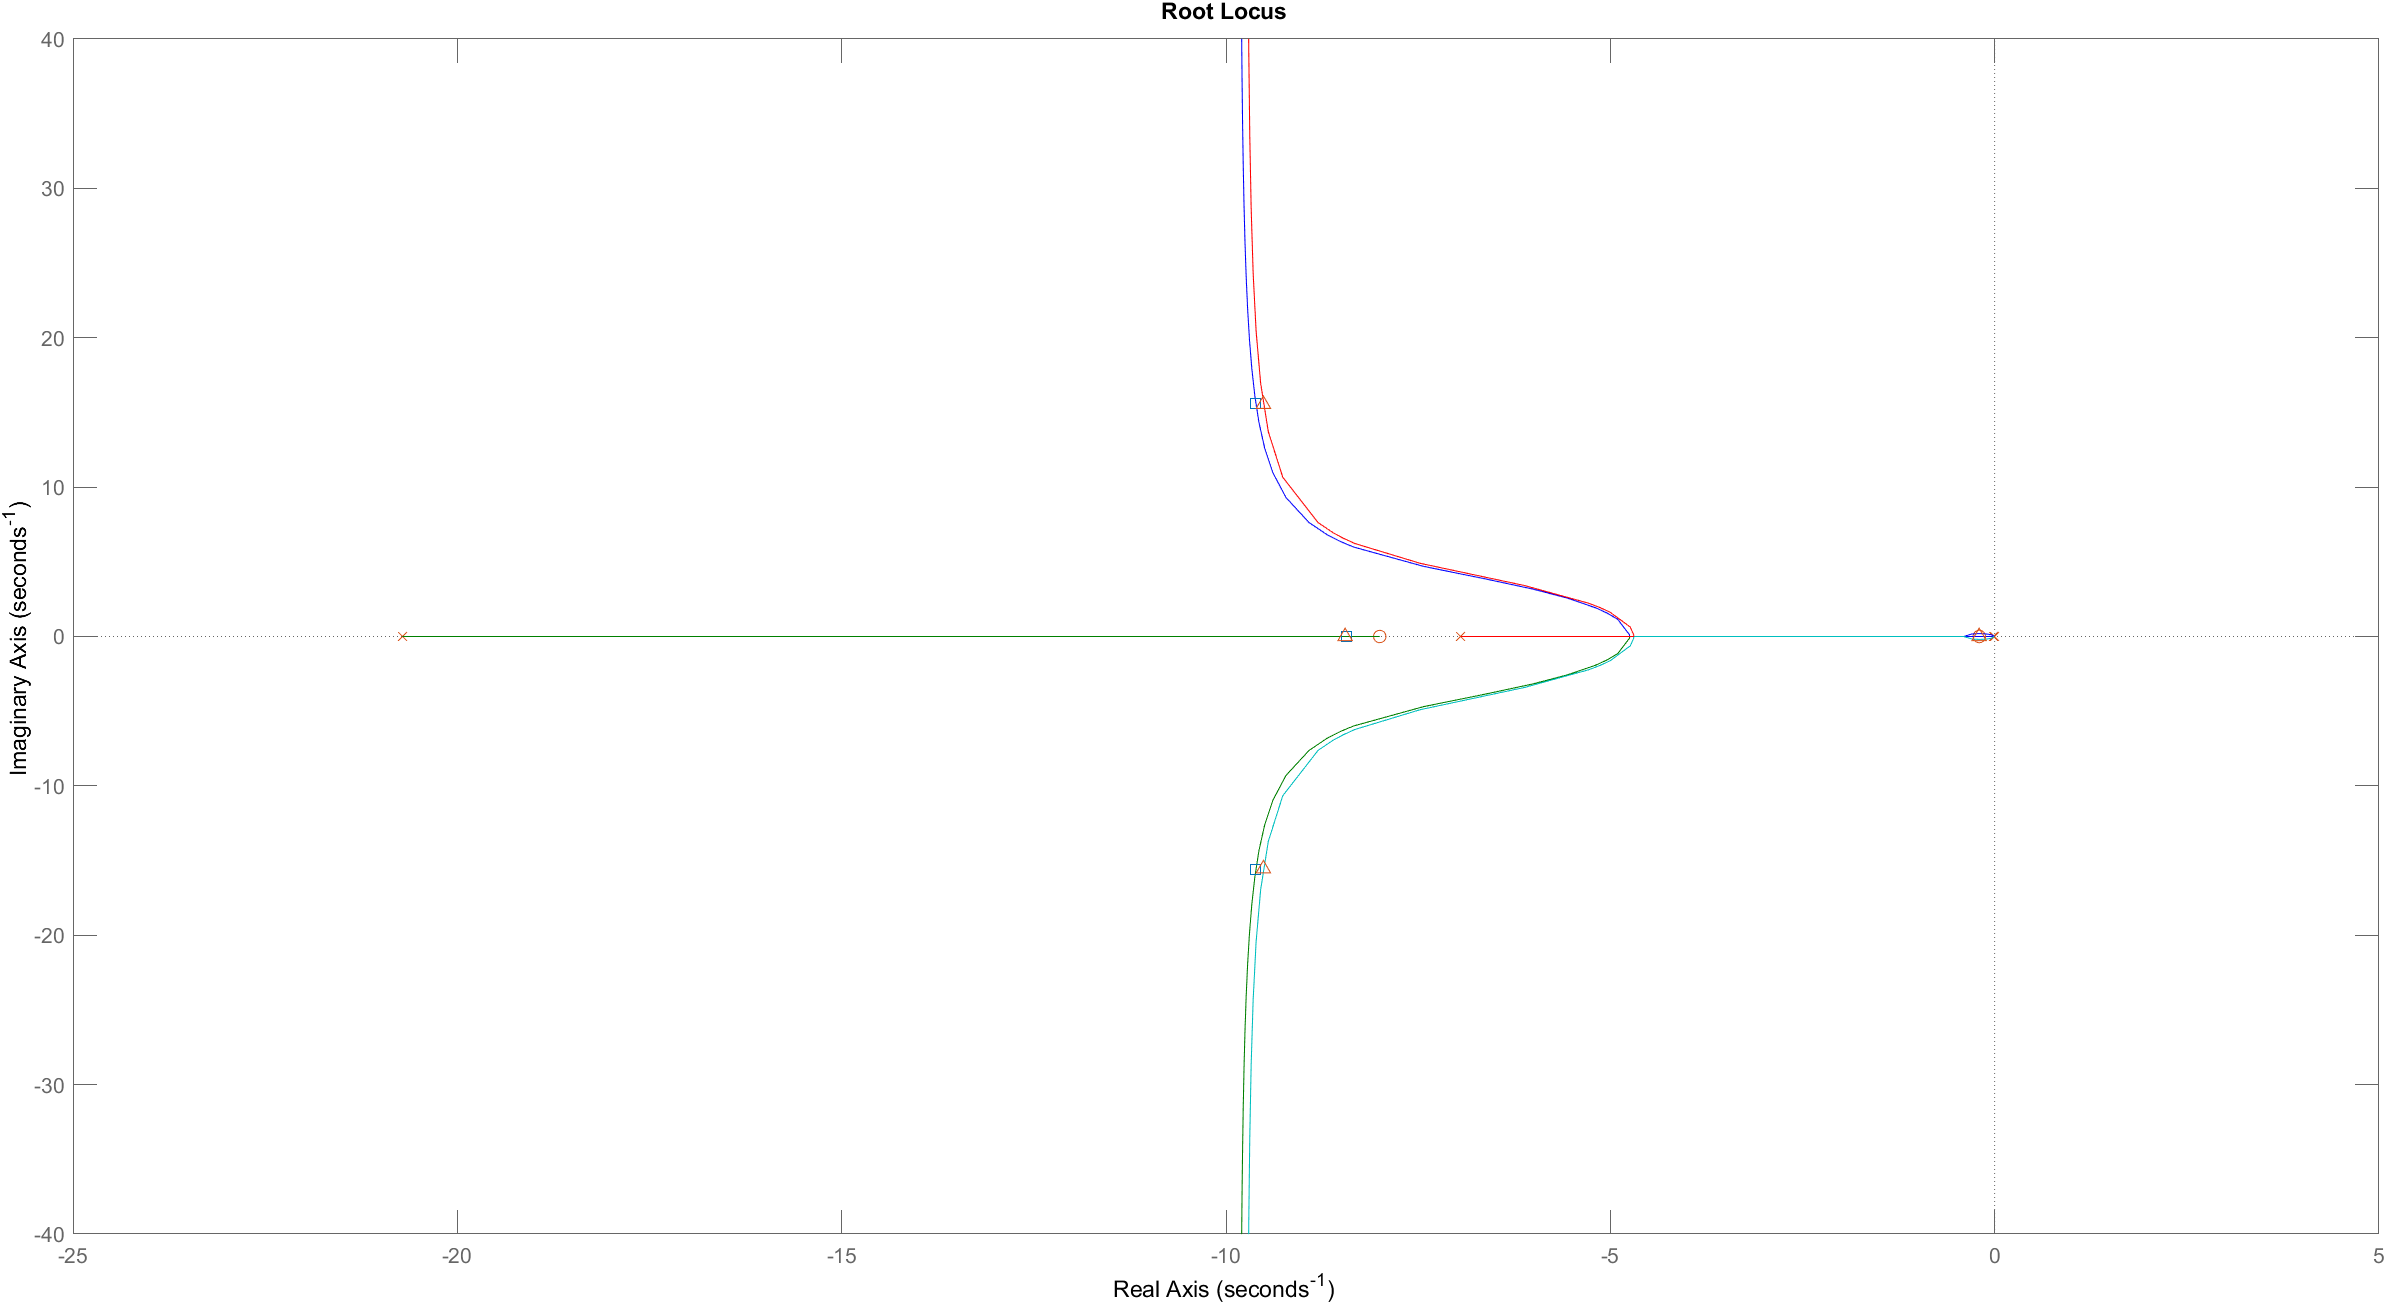
\includegraphics[width=\textwidth]{rlocus}
    \caption{\label{fig:rlocus}Root Locus}
\end{figure}

\begin{figure}[h]
    \centering
    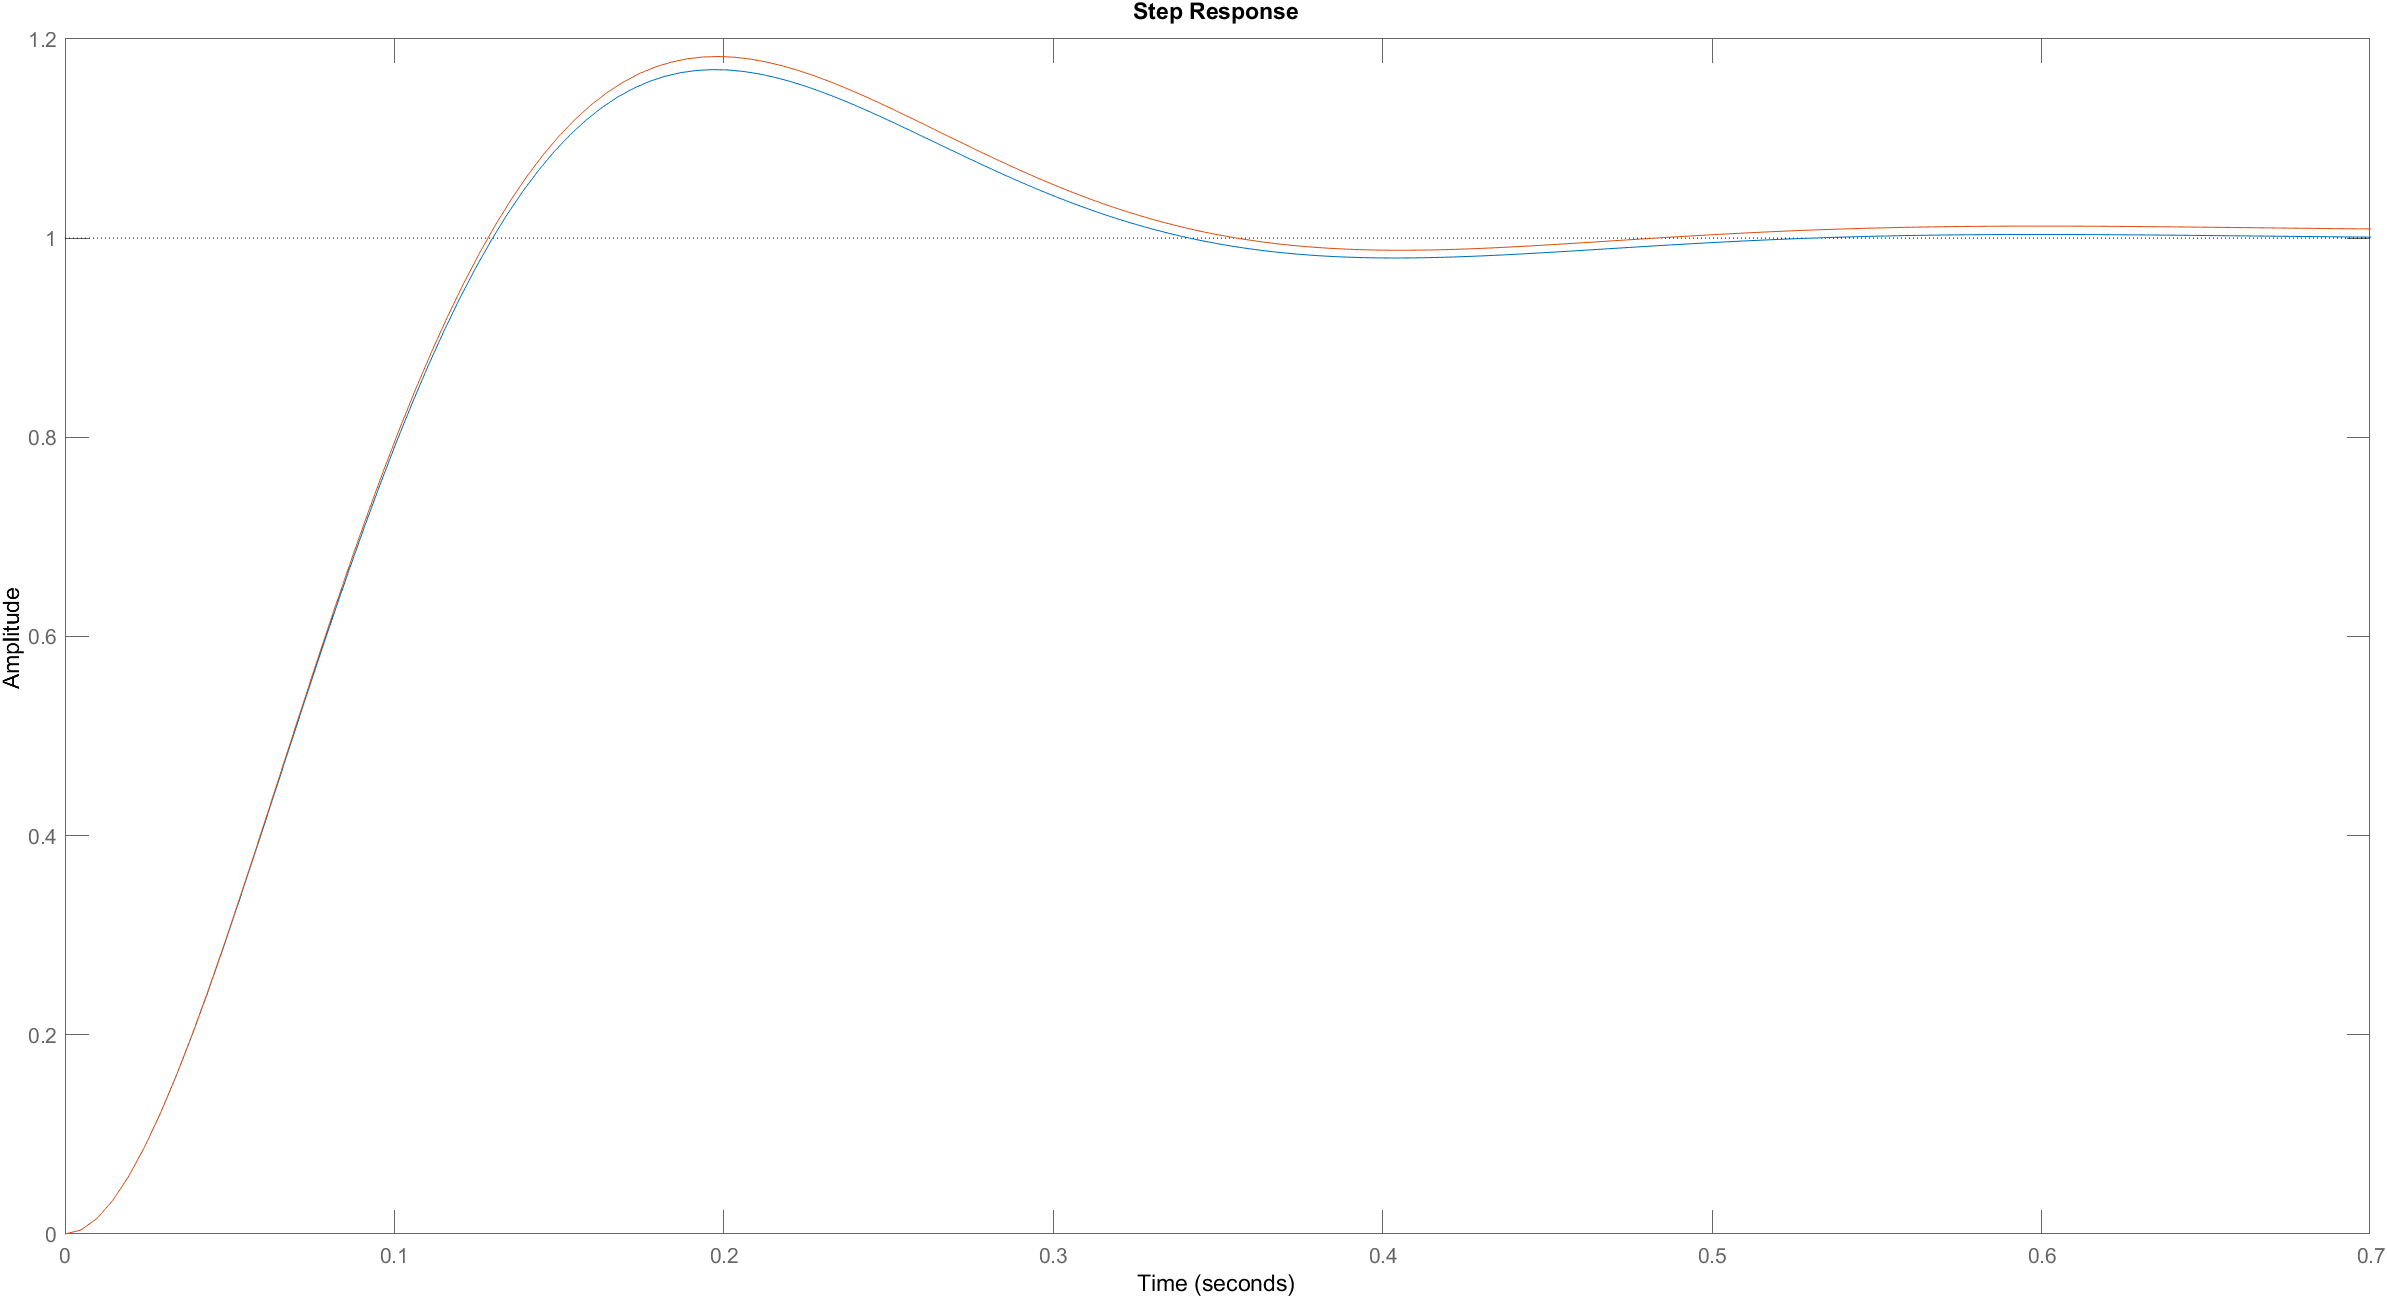
\includegraphics[width=\textwidth]{step_response}
    \caption{\label{fig:step}Step Response}
\end{figure}

\begin{figure}[h]
    \centering
    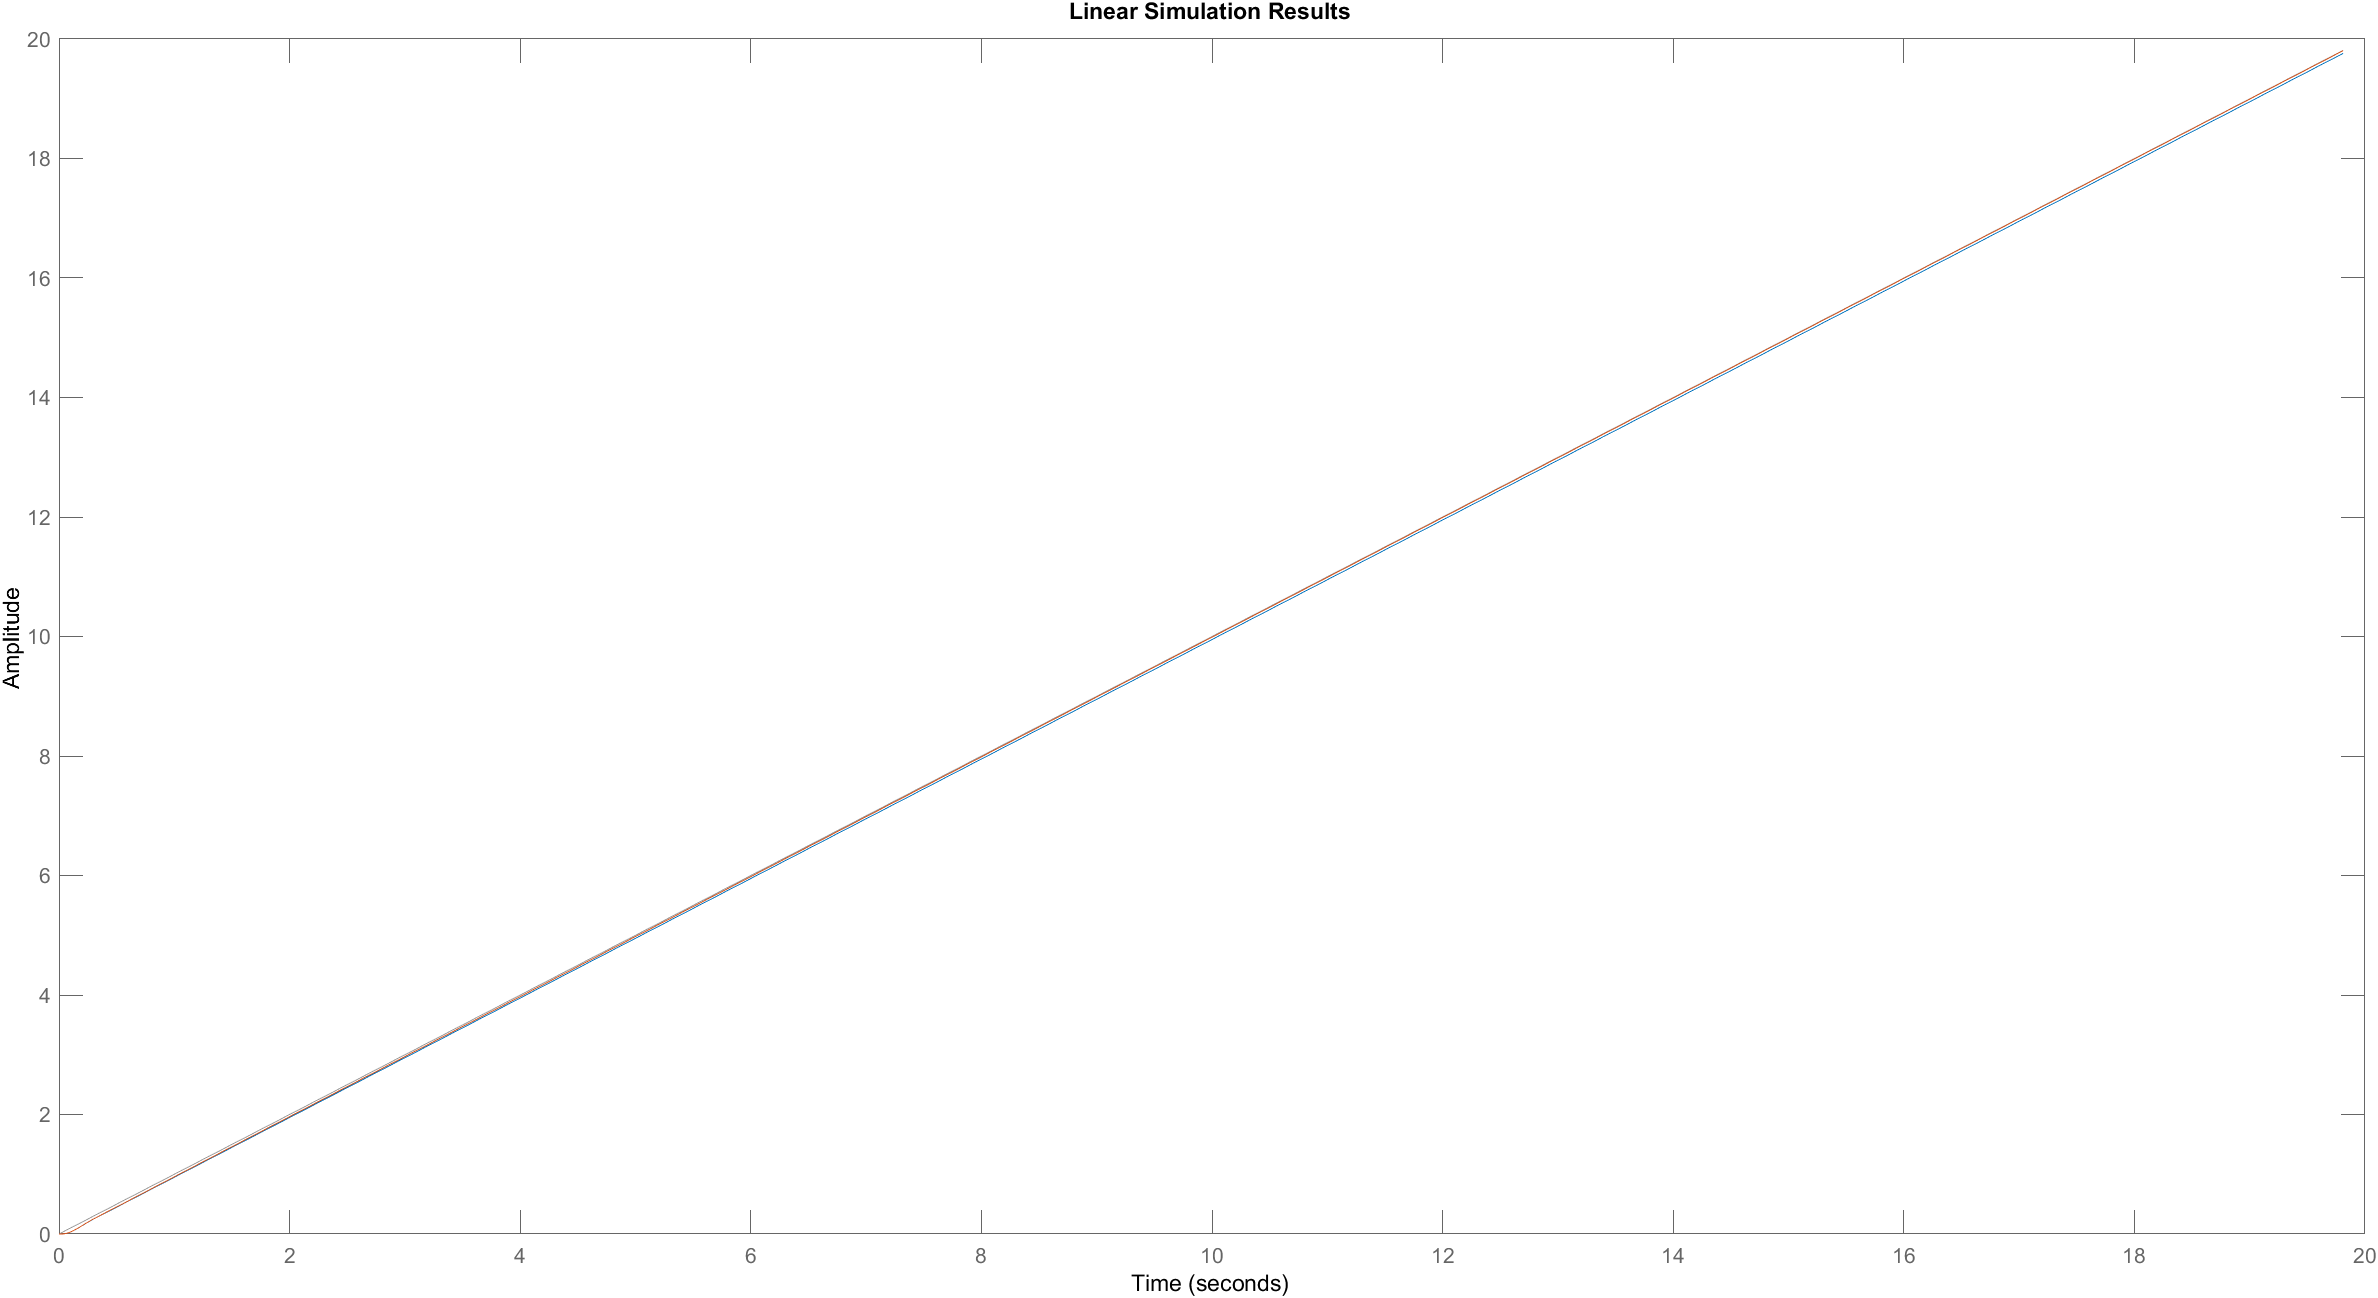
\includegraphics[width=\textwidth]{ramp_response}
    \caption{\label{fig:ramp}Ramp Response}
\end{figure}

\begin{figure}[h]
    \centering
    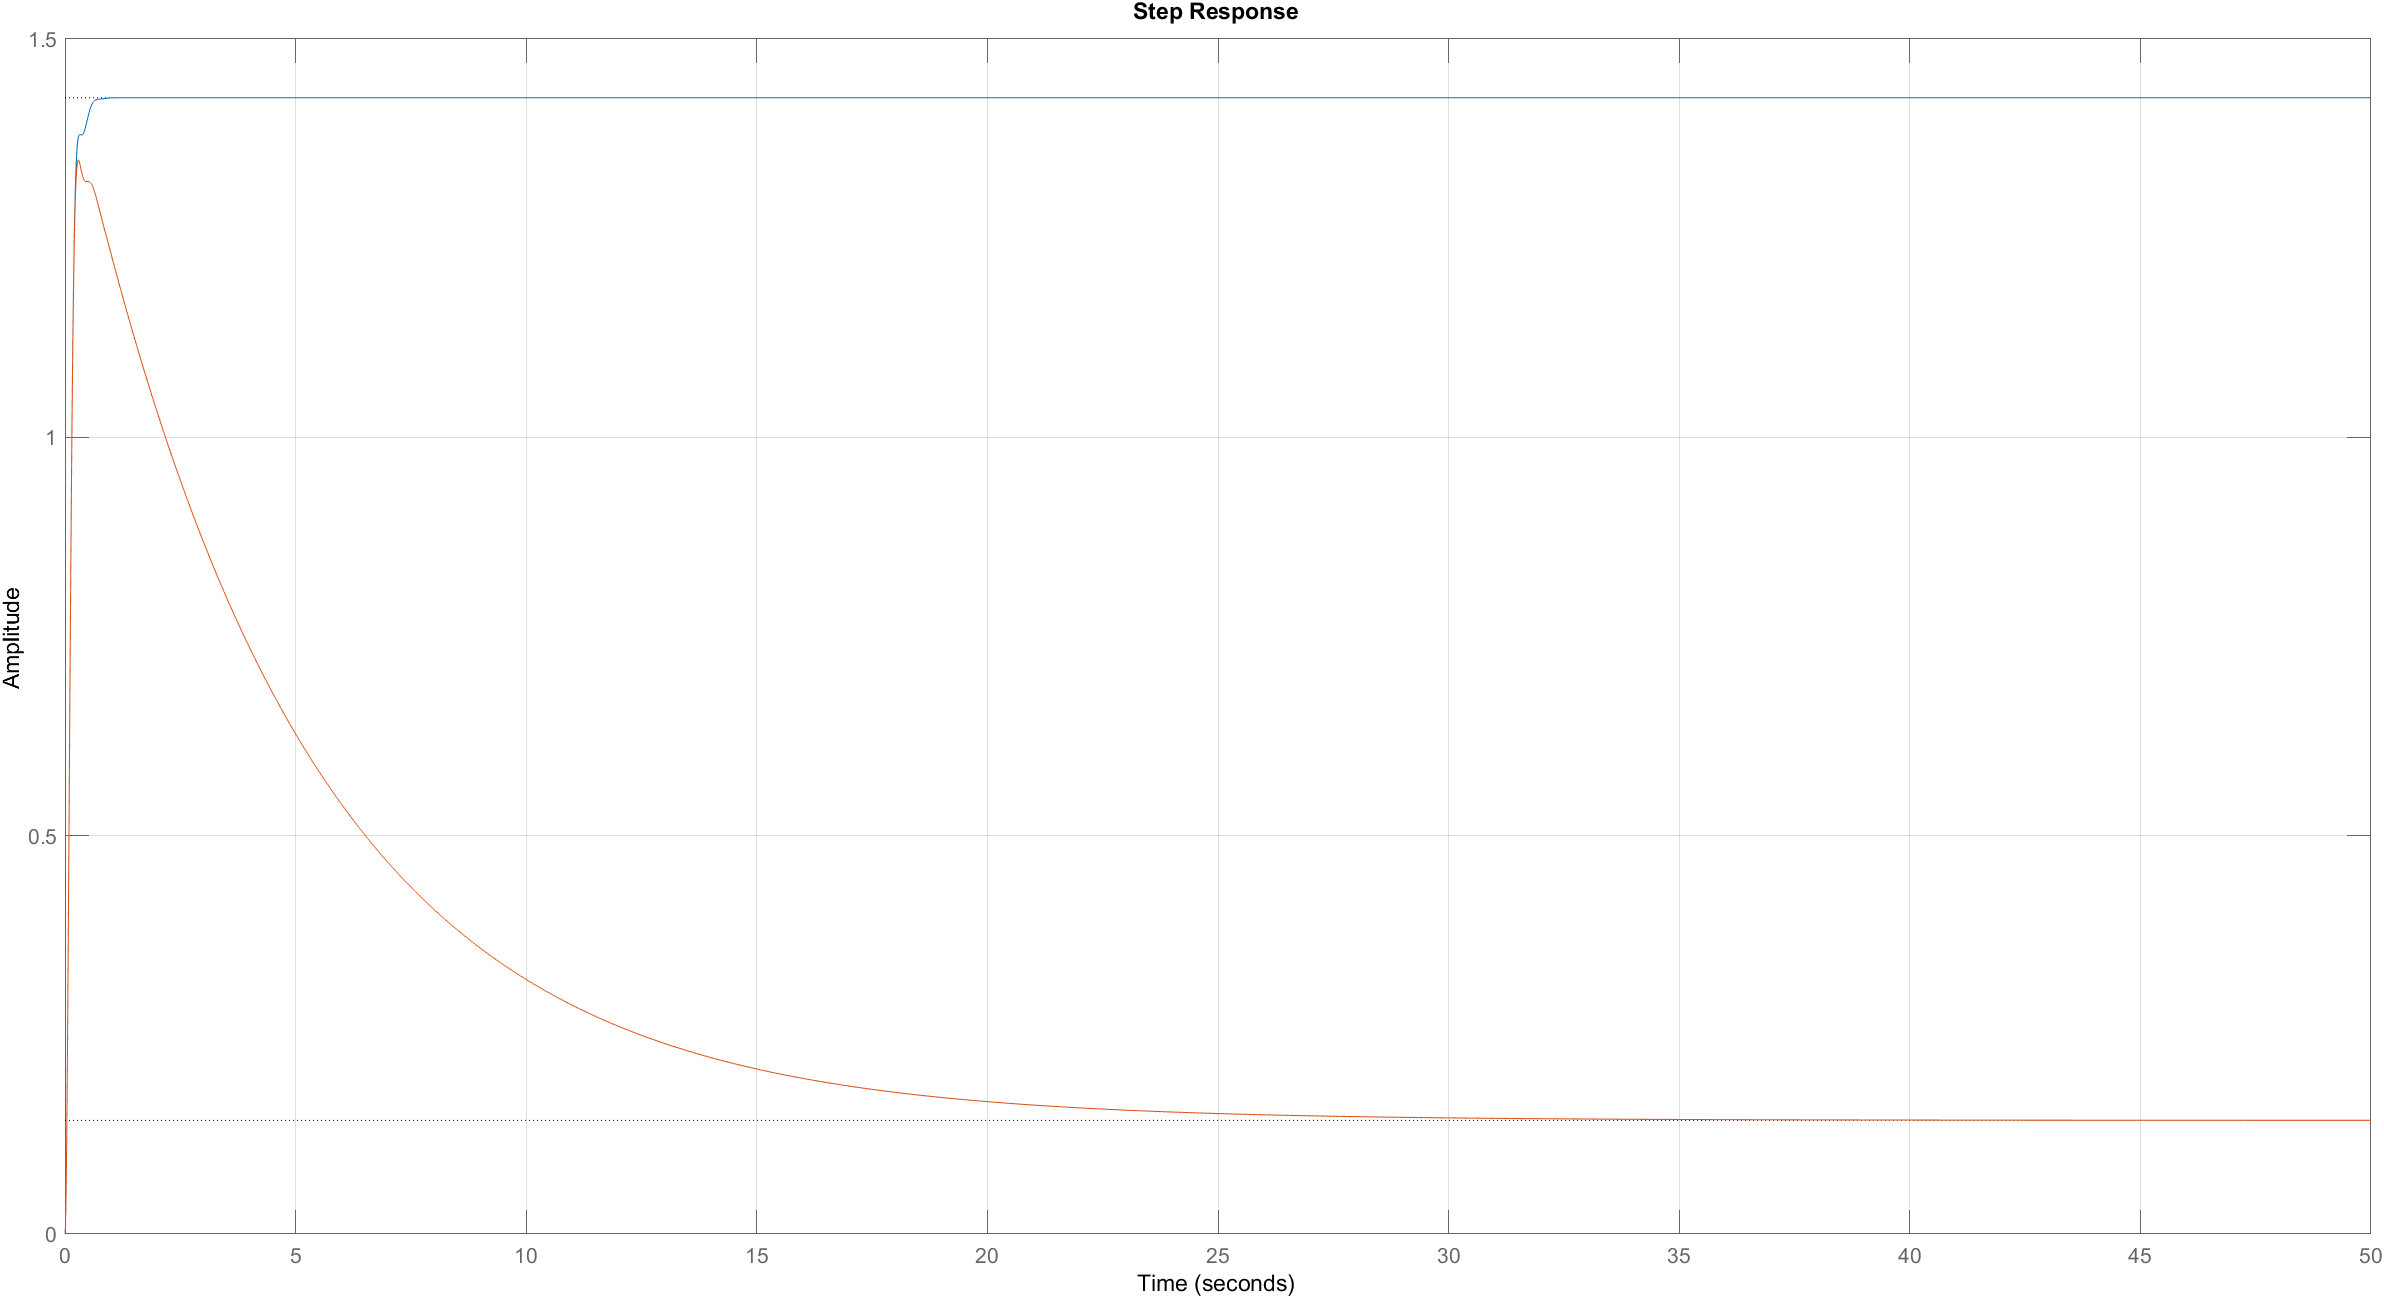
\includegraphics[width=\textwidth]{dist_response}
    \caption{\label{fig:dist}Step Disturbance}
\end{figure}

\clearpage

\section{Experiment: Implementation of Your Lead-Lag Compensator}

\end{document}